\documentclass[a4paper]{jpconf}
\usepackage{amsmath}
\usepackage{multirow}
\usepackage{graphicx}

\begin{document}
\title{Analyzing Human Behavior in Digitized Society: Insights from Wordle Data}


\author{Yitong Hu*}

\address{Beijing University of Posts and Telecommunications, Beijing, China}

\ead{huyt@bupt.edu.cn}

\author{Yizhe Wang*}

\address{Beijing University of Posts and Telecommunications, Beijing, China}

\ead{anonymity@bupt.edu.cn}

\author{Zixuan Zhu*}

\address{Beijing University of Posts and Telecommunications, Beijing, China}

\ead{ternura@bupt.edu.cn}

\begin{abstract}
This paper focuses on analyzing the human behavior of Wordle players using available player data. While there have been many studies discussing the mechanism, strategy, and cultural influence of Wordle, research on the relationship between player data and human group behavior is still lacking. The authors conducted a time series analysis of the number of daily Wordle players and developed a MIMO XGBoost model to predict the distribution of player attempts. The model demonstrates high confidence through a test set, and the authors analyze the predicted data to provide insights for game designers and sociologists.
\end{abstract}

\section{Introduction}
Wordle is a popular English word-guessing game created by Josh Wardle. Wordle generates a new and globally unique 5-letter word each day, and players need to guess the word in 6 attempts and can share their daily Wordle score on social media. After each guess, the system displays hints in different colors, including the letter in the correct position (green), with the letter but not in the guessed position (yellow), and without the letter (gray). wordle is simple to play, but fun and challenging, and has become popular on social media.

The explosion of Wordle has generated a lively discussion in the Internet community about word-guessing strategies. Players' discussions and summaries of word-guessing strategies may affect the distribution of players' scores. On the other hand, social media also influenced the daily game data. For example, the sharing of Wordle scores on social media may attract more people to play the game; players who guess the word of the day first may put hints on social media, which may reduce the difficulty of the game that day; or the hot events of a certain day may change the number of people playing Wordle that day, etc.\\
-----------------------------------------------------------------------\\
\scriptsize*In no particular order, the following are the first authors of the article.
\normalsize

Similarly, word-guessing games have attracted a great deal of attention in the academic community. Many studies have analyzed the popularity and user behavior of these games. For example, Teodoro F. Revano \cite{revano2018logical} investigates the factors that make word guessing games engaging and challenging, while Kasikrit Damkliang \cite{damkliang2016guessing} explores the social and cultural aspects of these games, focusing on how they reflect and shape language use. Other word-guessing games, such as Guess the Word and Word Association, have also been studied. k Smith \cite{smith2011cross} on word-guessing focuses on player strategies and game design, while Norbert Schmitt's \cite{schmitt1997researching} study on word association explores the cognitive processes behind word association and the potential of games for language learning.

However, Wordle's player data is not just related to the words themselves, but is a comprehensive representation of the behavior, mindset, and interaction patterns of human groups. Despite the widespread attention Wordle has received, our knowledge of its player behavior and score distribution is still limited. Therefore, we hope to reveal some interesting patterns and trends by analyzing Wordle's player data. We believe that research on such social media games can reveal broader social group phenomena and contribute to a better understanding of human behavior in a digital society.	

Driven by these goals, we study Wordle's daily player engagement counts and player score distributions, and explore the relationships between these data. First, we collected 359 days of Wordle and player data for the corresponding dates from the New York Times and Twitter. Based on our understanding of Wordle's rules and social network features, we propose heterogeneous spatio-temporal features that fuse word topology and social network activity. Secondly, we construct an Autoregressive Integrated Moving Average (ARIMA) model to analyze the number of players playing Wordle each day in a time-series and obtain predictions. Again, we propose a Multiple-input and Multiple-output Extreme Gradient Boosting (MIMO XGBoost) model to predict the distribution of players' scores and ensure that the distribution of scores satisfies the frequency sum constraint of 1. Finally, we analyze the correlation between the data and give the important factors influencing the player score distribution.

Through this study, we hope to provide valuable insights for game designers and sociologists to promote a better understanding of social group phenomena and human behavior in digital society.


\section{Data}
We extracted a total of 359 days of data from Twitter and the New York Times, and processed the datasets, including data integration, reduction, cleaning, and normalization. Data file entry descriptions are as follows:
\begin{itemize}
    \item {\bf Date: }The date in mm-dd-yyyy (month-day-year) format of a given Wordle puzzle.
    \item {\bf Word: }The solution word players are trying to guess on the associated date.
    \item {\bf Number of players: }The total number scores that were recorded on Twitter that day.
    \item {\bf n tries (1$\leq$ n $\leq$ 6): }The percentage of players solving the puzzle in n guesses.
    \item {\bf 7 or more tries (X): }The percentage of players that could not solve the puzzle in six or fewer tries. Note: the percentages may not always sum to 100\% due to rounding.

\end{itemize}

\subsection{Concept Definition}
\begin{enumerate}

    \item {\bf Solve (the Wordle puzzle): }Enter the correct letters in the correct order to form the Wordle word of the day.
    \item {\bf Distribution of the players’ score: }The associated percentages of (1, 2, 3, 4, 5, 6, X).

\end{enumerate}

\subsection{Problem Definition}
\begin{enumerate}

    \item {For the Number of players prediction problem, given a Date, output the predicted value of the Number of players on that day.}
    \item {For the prediction of the Distribution of the players' score problem, given a Word and a Date, output the prediction of the Distribution of the players' score for that word on that day. In other words, Predict 1 try, 2tries,... , 7 or more tries(X).}

\end{enumerate}

\subsection{Assumptions}
\begin{itemize}
    \item The records people post on Twitter are accurate.
    \item The data provided does not include incorrect data from competitors or malicious customers.
    \item The number of players recorded per day is equal to the sum of the number of statistics, i.e., there are no omitted or excluded records in any of the provided datasets.
    \item The record uploaded by the player was posted on the day of play.
    \item Each player uploads records at most once a day.
\end{itemize}






\section{Methodology} 
\subsection{Spatio-Temporal Feature Extraction}
In order to complete the above two prediction problems, we need more attributes to build our model \cite{yuan2021survey}, \cite{siami2019performance}. According to the rules of Wordle and the characteristics of social networks, we extract the features of the data from two dimensions of space and time.


In the {\bf spatial dimension}, Wordle is an alphabet-oriented English word puzzle game, which determines that the topology of words greatly affects the distribution of the number of attempts of human players \cite{sheng2022optimized}, \cite{zhu2022application}. Based on the analysis of Wordle recipes on social networking sites and the morpheme formation of English words, we propose to use the Table~\ref{notation} features to measure the topology of words:
\begin{center}
\begin{table}[h]
\centering
\caption{\label{notation}Notations} 
\begin{tabular}{@{}l*{15}{l}}
\br
Element&Definition\\
\mr
    $PS$ &The part of speech.\\
    $R_{tn }$ &The percentage of players solving the puzzle in n guesses.\\
    $F$ &Word frequency\\
    $N_{dw}$ &The number of duplicate letters\\
    $N_v$ &The number of vowels\\
    $N_c$ &The number of consonants\\
    $N_{iw}$ &The number of infrequently used words\\
    $N_s$ &The number of syllables\\
    $IF_{rc}$ &Repetition is continuous or not\\
    $IF_{vb}$ &Vowel beginning or not\\
    $IF_{ve}$ &Vowel ending or not\\
    $IF_{vc}$ &Vowel is continuous or not\\
    $IF_{p}$ &Polysemous or not\\
\br
\end{tabular}
\end{table}
\end{center}

In the {\bf time dimension}, the activity of the social network may affect the number of participants in the game and the level structure of players, which in turn may affect the distribution of the number of attempts \cite{wang2020forecasting}. We select the trading day data of the New York Stock Exchange to mark the date, and introduce the feature Workday or not as a representation of social network activity.

In summary, we propose a heterogeneous spatiotemporal feature that combines word topology and social network activity, and follow the principle of data standardization for quantitative processing to obtain quantitative and categorical (starting with IF) features.


\subsection{ARIMA Model}
The autoregressive model describes the relationship between the current value and the historical value and uses the historical time data of the variable to predict itself.

In general, the formula of the P-order autoregressive process is defined as follows:
\begin{equation}\label{eq:AR_1}
    y_{t}=\mu+\sum_{i=1}^{p} \gamma_{i} y_{t-i}+\epsilon_{t}
\end{equation}
Where $y_t$ is the current value, $\mu$ is the constant term, $p$ is the order, $r_i$ is the autocorrelation coefficient, and $\epsilon_t$ is the error.


General P-order autoregressive model AR:
\begin{equation}\label{eq:AR_2}
    x_{t}=\alpha_{1} X_{t-1}+\alpha_{2} X_{t-2}+\ldots+a_{p} x_{t-p}+\mu_{t}
\end{equation}

As can be seen from the formula, the current value is predicted by the historical value, and p is an order in the autoregressive model, which indicates that the historical value of several epochs is used to predict the current value.

Moving averages focus on the accumulation of error terms in autoregressive models.

Among them, the formula of the q-order self-MA model is defined as follows:
\begin{equation}\label{eq:MR_1}
    y_{t}=\mu+\epsilon_{t}+\sum_{i=1}^{q} \theta_{i} \epsilon_{t-i}
\end{equation}

In the AR model, if it is not white noise, it is usually considered to be a moving average of order q:
\begin{equation}\label{eq:MR_2}
u_{t}=\varepsilon_{t}+\beta_{1} \varepsilon_{t-1}+\ldots+\beta_{q} \varepsilon_{t-q}
\end{equation}

The moving average method can effectively eliminate random fluctuations in the forecast \cite{siami2018comparison}.
The autoregressive moving average model consists of two parts: the autoregressive part and the moving average part. The regression equation is expressed as follows:
\begin{equation}\label{eq:ARMA}
    y_{t}=\mu+\sum_{i=1}^{p} \gamma_{i} y_{t-i}+\epsilon_{t}+\sum_{i=1}^{q} \theta_{i} \epsilon_{t-i}
\end{equation}


It can be seen from the regression equation that the autoregressive moving average model combines the advantages of AR and MA. In the ARMA model, the autoregressive process is responsible for quantifying the relationship between the current data and the previous data, and the moving average process is responsible for solving the problem of random changes.

The Autoregressive model (AR), the moving average model (MA), and the difference method (I) are combined to obtain the differential autoregressive moving average model ARIMA (p, d, q), where d is the order of the difference to be performed on the data, and ARIMA \cite{kalpakis2001distance} is the ARMA model after the difference.








\subsection{MIMO XGBoost Model}

\subsubsection{Traditional XGBoost Model}
First, we analyze the traditional XGBoost Model \cite{chen2016xgboost}: A tree ensemble model consists of a set of classification and regression trees (CART). Mathematically speaking, we can write the model as follows:
\begin{equation}\label{eq:1}
    \hat{y}_{i}=\sum_{k=1}^{K} f_{k}\left(x_{i}\right), f_{k} \in \mathcal{F}
\end{equation}

Among them, the K is the number of trees, f is a function of f space, f it is possible to set the CART, the input value $\vec{x_i}=\{IF_{rc},f,N_{dw},N_v,N_c,N_iw,N_s,IF_{vb},IF_{vc},IF_p,IF_w\}$. The objective function of the above model is given by the following equation:
\begin{equation}\label{eq:3}
    \operatorname{obj}(\theta)=\sum_{i}^{n} l\left(y_{i}, \hat{y}_{i}\right)+\sum_{k=1}^{K} \omega\left(f_{k}\right)
\end{equation}

Where the first term is the loss function, and the second term is the regularization parameter.


For the current tree model, the learning method is to define the objective function and optimize it. We have defined the objective function above, but considering the difficulty of learning the tree structure, we also adopt the addition strategy to optimize it, adding a new tree at a time:

\begin{equation}\label{eq:3}
\hat{y}_i^{(t)} = \sum_{k=1}^t f_k(x_i)= \hat{y}_i^{(t-1)} + f_t(x_i)
\end{equation}


Then select the tree that can optimize the objective function, and consider using the mean square error (MSE) as the loss function:

\begin{equation}\label{eq:origin}
\begin{split}\text{obj}^{(t)} & = \sum_{i=1}^n (y_i - (\hat{y}_i^{(t-1)} + f_t(x_i)))^2 + \sum_{i=1}^t\omega(f_i) \\
          & = \sum_{i=1}^n [2(\hat{y}_i^{(t-1)} - y_i)f_t(x_i) + f_t(x_i)^2] + \omega(f_t) + \mathrm{constant}\end{split}
\end{equation}

The loss function is obtained by Taylor expansion to second order and removing all constants:
\begin{equation}
\sum_{i=1}^n [g_i f_t(x_i) + \frac{1}{2} h_i f_t^2(x_i)] + \omega(f_t)
\end{equation}

Under this definition, the value of the objective function is determined only by $g_i$ and $h_i$. This is how XGBoost supports custom loss functions.


After reformulating the tree model, we can write the target value as:

\begin{equation}
\begin{split}\text{obj}^{(t)} &\approx \sum_{i=1}^n [g_i w_{q(x_i)} + \frac{1}{2} h_i w_{q(x_i)}^2] + \gamma T + \frac{1}{2}\lambda \sum_{j=1}^T w_j^2\\
&= \sum^T_{j=1} [(\sum_{i\in I_j} g_i) w_j + \frac{1}{2} (\sum_{i\in I_j} h_i + \lambda) w_j^2 ] + \gamma T\end{split}
\end{equation}

If the structure part q of the tree is known, the objective function can be used to find the optimal Wj and obtain the optimal objective function value. Its essence can be reduced to the problem of solving the minimum value of quadratic function. The solution is:
\begin{equation}
\begin{split}w_j^\ast &= -\frac{G_j}{H_j+\lambda}\\
\text{obj}^\ast &= -\frac{1}{2} \sum_{j=1}^T \frac{G_j^2}{H_j+\lambda} + \gamma T\end{split}
\end{equation}

\subsubsection{New MIMO XGBoost Model}
The traditional XGBoost model \cite{chen2016xgboost} is a multi-input single-output model that can only predict the value of one n tries ($R_{tn}$) at a time. If  seven XGBoost models are trained independently, the different $R_{tn}$ may not satisfy the following constraints due to the lack of correlation:
\begin{equation}
\text { total }=\sum_{n=1}^{7} R_{t n}=100
\end{equation}

To address the above challenges, we propose the MIMO XGBoost model (see Figure~\ref{fig:model}). We train seven XGBoost regression models synchronously to predict the player score distribution (the value of $R_{t1}-R_{t7}$) based on word's spatio-temporal properties, i.e., MIMO. Furthermore, a distributed objective function is designed to ensure that the seven models optimize the parameters towards a common goal, that is, the constraint that the sum of frequencies is 1 is satisfied. After the joint training is completed, each model can be used independently, that is, asynchronously. Specifically, the data of the seven XGBoost models are shared and the iterations are synchronized. After each round of iteration, the Synchro-Aggregation Controller collects the output values of the seven models and sends the seven values to each model, and then informs all the models for the next round of iteration. In other words, the Controller enables the sharing of output values between models and synchronization of training.

\begin{figure}[htbp]
    \centering
    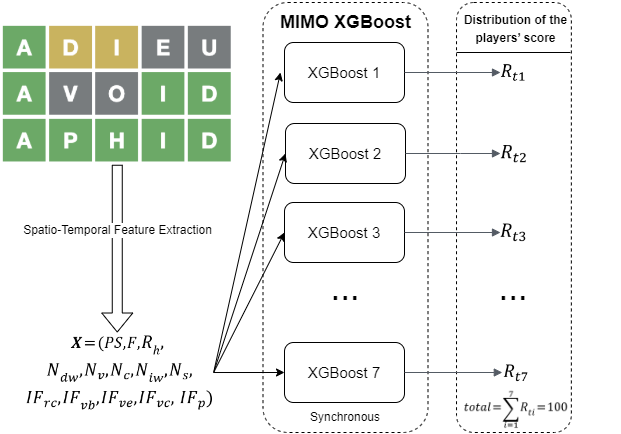
\includegraphics[width=.7\textwidth]{img/model.png}
    \caption{MIMO XGBoost Model}\label{fig:model}
\end{figure}

Correspondingly, model n is used to predict $R_{tn}$. For each data point i in model n, we add a bias term to the square loss $V_{dn}$:
\begin{equation}
\begin{array}{c}
\operatorname{Loss}_{n}=\left(y_{n i}-\hat{y}_{n i}\right)^{2}+V_{d n} \\
V_{d n}=10^{-2} y_{n i}\left(100-\sum_{j=1}^{7} \hat{y}_{j i}\right)^{2}
\end{array}
\end{equation}

Where, $y_{in}$ denotes the value of n tries for data point i. Accordingly, $\hat{y}_{ji}$ represents the predicted value of j tries for data point i. Since the overall deviation $(100-\sum_{j=1}^{7} \hat{y}_{j i})$ is the result of the combined effect of 7 models, the overall deviation is multiplied by the contribution coefficient $10^{-2}y_{ni}$ to obtain the contribution of model n in the overall deviation. That is, the bias $V_{dn}$ caused by model n.
Next, we define the cost function for model n:
\begin{equation}
\operatorname{Cost}_{n}=\sum_{i}^{N} \operatorname{Loss}_{n}=\sum_{i}^{N}\left[\left(y_{n i}-\hat{y}_{n i}\right)^{2}+10^{-2} y_{n i}\left(100-\sum_{j=1}^{7} \hat{y}_{j i}\right)^{2}\right]
\end{equation}


Where N is the total number of data points in the training set.
We pick the vector $X=\left(P S, F, R_{h}, N_{d w}, N_{v}, N_{c}, N_{i w}, N_{s}, I F_{r c}, I F_{v b}, I F_{v e}, I F_{v c}, I F_{p}\right)$ as input, the model of n, in its own namespace, has the following objective function:

\begin{equation}
\begin{split}
    \mathrm{obj}_{n}^{(t)} & =\operatorname{Cost}_{n}+\sum_{i=1}^{t} \omega\left(f_{k}\right) \\
& =\sum_{i=1}^{N}\left[2\left(\hat{y}_{n i}^{(t-1)}-y_{n i}\right) f_{t}\left(\boldsymbol{X}_{i}\right)+f_{t}\left(\boldsymbol{X}_{i}\right)^{2}+10^{-2} y_{n i}\left(100-\sum_{j=1}^{7} \hat{y}_{j i}\right)^{2}\right]+\omega\left(f_{t}\right)+\text { constant }
\end{split}
\end{equation}

Taking the Taylor expansion of the loss function to second order and removing all the constants yields:
\begin{equation}
\operatorname{obj}_{n}^{(t)}{ }= \sum_{i=1}^{N}\left[g_{i} f_{t}\left(\boldsymbol{X}_{i}\right)+\frac{1}{2} h_{i} f_{t}^{2}\left(\boldsymbol{X}_{i}\right)\right]+\omega\left(f_{t}\right)
\end{equation}

The value of the objective function only depends on $g_i$ and $h_i $. In line with the way XGBoost supports custom loss functions.




\section{Results \& Discussion}



\subsection{ARIMA Model Checking}
We finally determined the ARIMA model as ARIMA(1,1,0), and then substituted the standardized data set. The model parameter table is as follows. The Table \ref{A} shows the results of this model test, including the number of samples, degrees of freedom, Q statistics and the goodness of fit of the information criterion model. According to the test table, the goodness of fit R² of the model is 0.977, and the model perform well.
% Table
%\usepackage{multirow}
\begin{table}[]
\centering
\begin{tabular}{|ccc|}
\hline
\multicolumn{3}{|c|}{ARIMA   model (1,1,0) Test Table}                                          \\ \hline
\multicolumn{1}{|c|}{Item}              & \multicolumn{1}{c|}{Symbol}         & Value           \\ \hline
\multicolumn{1}{|c|}{}                  & \multicolumn{1}{c|}{Df   Residuals} & 45              \\ \hline
\multicolumn{1}{|c|}{Number of samples} & \multicolumn{1}{c|}{N}              & 48              \\ \hline
\multicolumn{1}{|c|}{\multirow{5}{*}{Q statistic}}           & \multicolumn{1}{c|}{Q6(P   value)} & 3.317(0.069*) \\ \cline{2-3} 
\multicolumn{1}{|c|}{}                  & \multicolumn{1}{c|}{Q12(P value)}   & 13.838(0.031**) \\ \cline{2-3} 
\multicolumn{1}{|c|}{}                  & \multicolumn{1}{c|}{Q18(P value)}   & 18.141(0.111)   \\ \cline{2-3} 
\multicolumn{1}{|c|}{}                  & \multicolumn{1}{c|}{Q24(P value)}   & 18.315(0.435)   \\ \cline{2-3} 
\multicolumn{1}{|c|}{}                  & \multicolumn{1}{c|}{Q30(P value)}   & 18.384(0.784)   \\ \hline
\multicolumn{1}{|c|}{\multirow{2}{*}{Information criterion}} & \multicolumn{1}{c|}{AIC}           & 1041.317      \\ \cline{2-3} 
\multicolumn{1}{|c|}{}                  & \multicolumn{1}{c|}{BIC}            & 1046.867        \\ \hline
\multicolumn{1}{|c|}{Goodness of fit}   & \multicolumn{1}{c|}{R²}             & 0.977           \\ \hline
\end{tabular}
\caption{\label{A}Note: ***, **, * represent significance levels of 1\%, 5\%, and 10\% respectively}
\end{table}


Finally, we got the time series diagram and prediction interval diagram for the simulated average number of people, as shown in the Figure \ref{fig:TSP} and Figure \ref{fig:end}:

\begin{figure}[h]
\begin{minipage}{20pc}
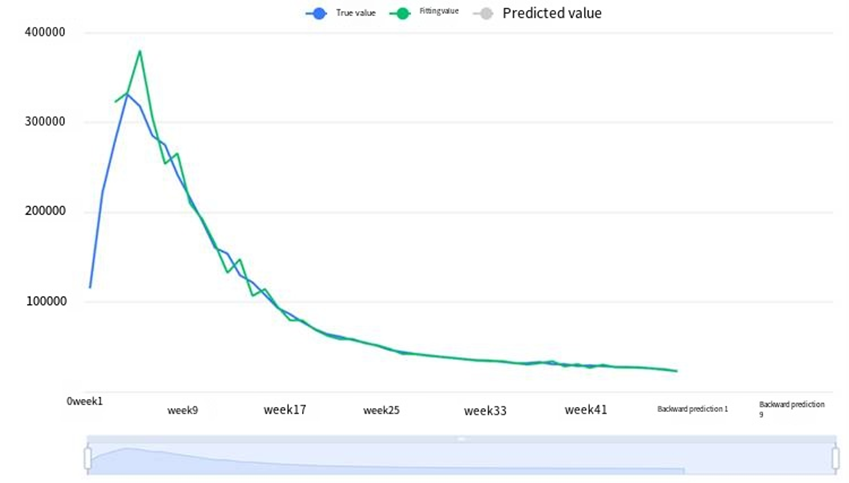
\includegraphics[width=20pc]{img/TSP.png}
\caption{\label{fig:TSP}Time series graph of average population}
\end{minipage}\hspace{2pc}%
\begin{minipage}{20pc}
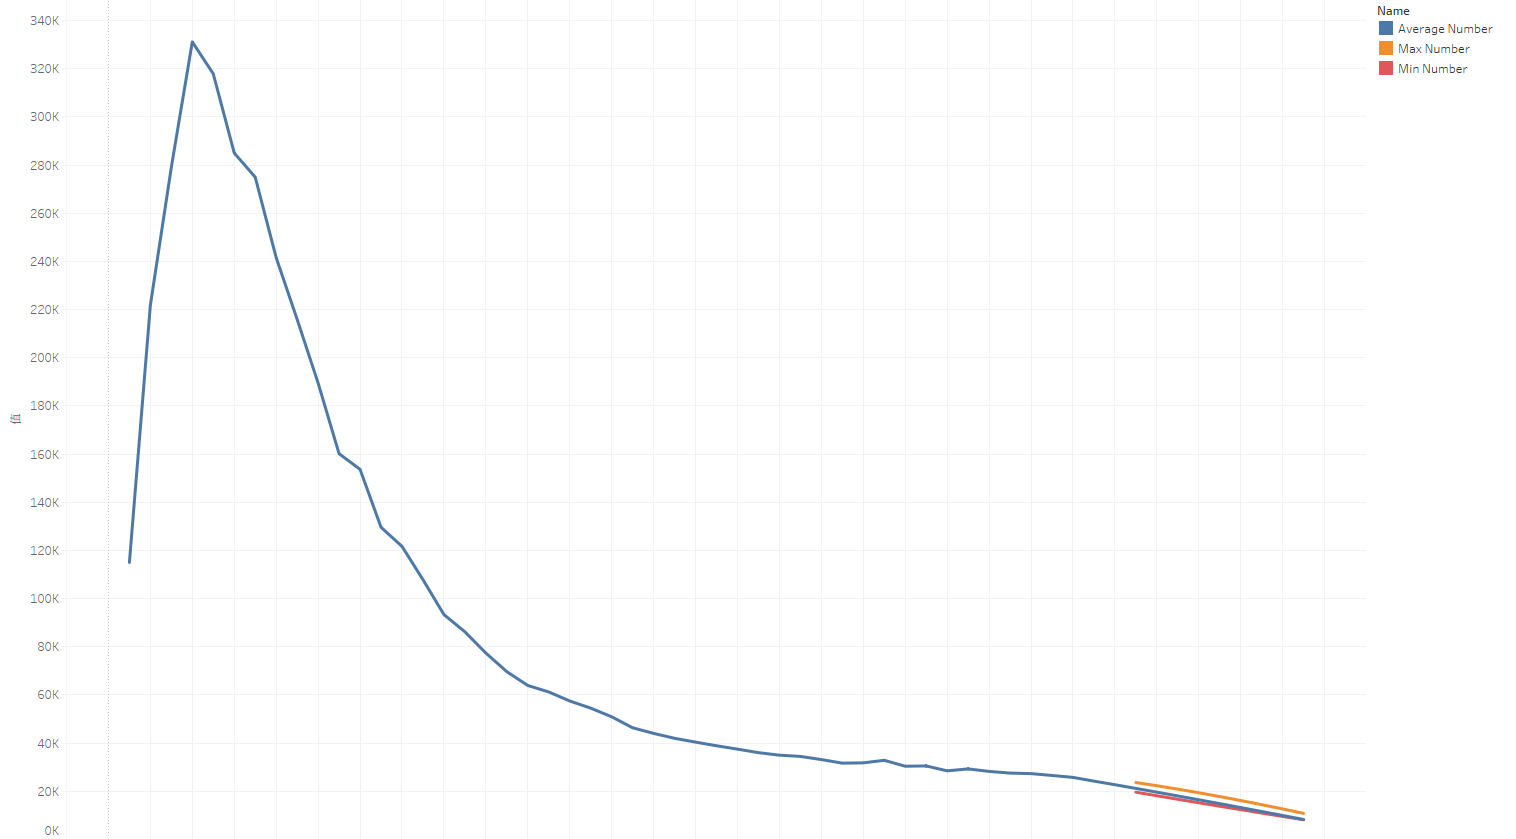
\includegraphics[width=20pc]{img/end.png}
\caption{\label{fig:end}The forecast range of the average population}
\end{minipage} 
\end{figure}




It can be seen that through the ARIMA Model, the time-related group phenomenon of the number of players can be accurately predicted.




\subsection{MIMO XGBoost Model Detection}


Using 70\% of the normalized dataset as the training set and the remaining part as the test set, the Percentage of the n tries($R_{tn}$) of the test set is calculated, and the predicted values of each are obtained, in Table i, the left side is the predicted value and the right side is the true value.

\begin{figure}[htbp]
\centering
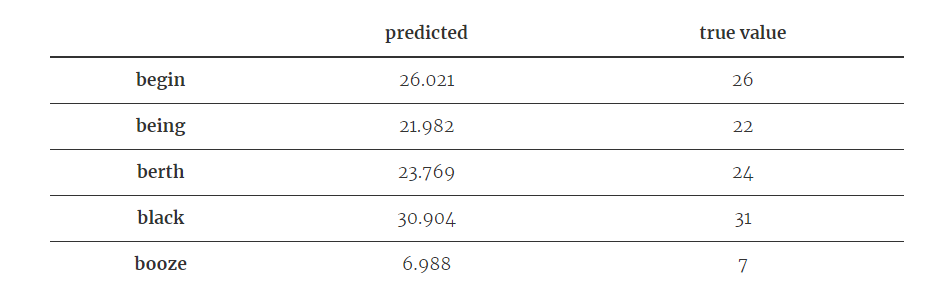
\includegraphics[width=.7\textwidth]{img/image.png}
\caption{\label{fig:image}3 tries Partial table of test samples versus real samples}
\end{figure}

As can be seen from the Figure \ref{fig:image}, the difference between all predicted and true results is very small, at most 0.24.

Carrying out our quantitative tests using several common statistical parameters for the obtained data conclusions, Root Mean Square Error (RMSE) is the first measure we choose to use, which can effectively test the accuracy of the predicted values, the relevant formula is as follows:

\begin{equation}\label{eq:RMSE}
R M S E=\sqrt{\frac{1}{n} \sum_{i=1}^{n}\left(\hat{y}_{i}-y_{i}\right)^{2}}
\end{equation}

In addition, we choose the Mean Absolute Error (MAE) as the accuracy measure. MAE can reflect the actual situation of the predicted value error, and the relevant formula is as follows:

\begin{equation}\label{eq:MAE}
\mathrm{MAE}=\frac{1}{\mathrm{n}} \sum_{\mathrm{i}=1}^{\mathrm{n}}\left|\hat{\mathrm{y}}_{\mathrm{i}}-\mathrm{y}_{\mathrm{i}}\right|
\end{equation}

Finally, the conventional goodness-of-fit $R^2$ is selected as the overall evaluation of model fitting. The Figure \ref{fig:compare} shows the test result statistics of the test set and the training set:

\begin{figure}[htbp]
\centering
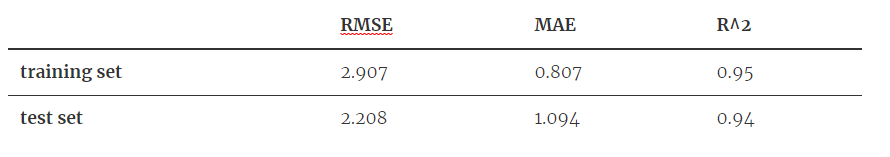
\includegraphics[width=.8\textwidth]{img/compare.png}
\caption{Evaluation results of EERIE}\label{fig:compare}
\end{figure}

The evaluation indexes of the training set were $RMSE=2.907$ , $MAE=0.807$,$R^2=0.95$ It can be considered that our optimized model has a good fit.
The evaluation metrics for the test set were RMSE = 2.208 and MAE = 1.094, respectively, with a goodness of fit, indicating that the predictiveness of the model is very accurate and reflects the influence of the objective property of words on the distribution of attempts.


\subsection{Discussion}

\begin{figure}[h]
\begin{minipage}{18pc}
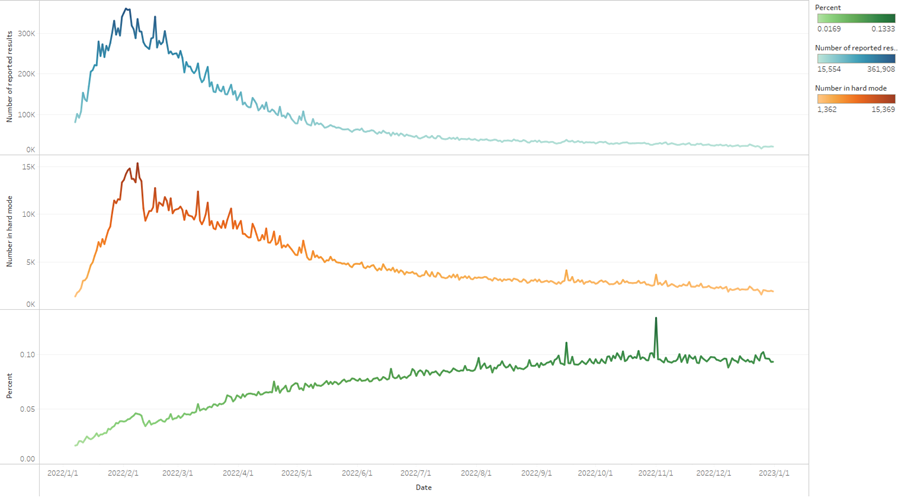
\includegraphics[width=24pc]{img/insight1.png}
\caption{\label{fig:insignt1}Trends in three kinds of data}
\end{minipage}\hspace{2pc}%
\begin{minipage}{18pc}
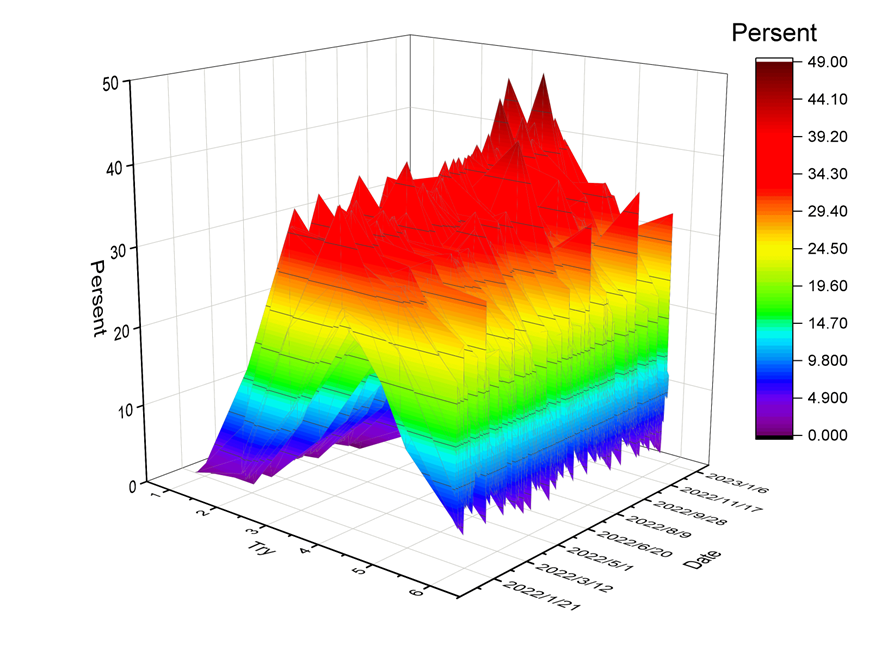
\includegraphics[width=20pc]{img/insight2.png}
\caption{\label{fig:insignt2}The variation trend}
\end{minipage} 
\end{figure}


In addition, through the study of the data, we found the characteristics that are reflected in the data. Figure \ref{fig:insignt1} shows the data graphs of the number of people who participated in the game, the number of people who chose the difficult mode, and the percentage of the number of people who chose the difficult mode to the total number of people over time, respectively. From the graph, we can easily see that the number of people playing each day shows a trend of increasing and then decreasing. At the same time, we notice that the percentage of difficult mode players is increasing slightly, which, combined with the two graphs above, we can roughly assume is mainly caused by the decrease in the total number of players, but this percentage also reflects that there are still a group of loyal users of difficult mode who are eager to challenge themselves in the word-guessing game every day. Figure \ref{fig:insignt2} reflects the numerical relationship between the number of attempts, date and percentage, which is roughly normally distributed, with the daily highs in percentage concentrated between 2, 3, 4 and 5 attempts. All cases of 1 vs. 7 attempts can be considered as having a very low percentage when excluding the anomalies of individual players, and this feature is well corroborated with our previous predictions for words.


\section{Conclusion}
We looked at Wordle's daily Number of players and Number of players and explored the relationship between these data. First, we collected 359 days of player data for words and corresponding dates from the New York Times and Twitter. Based on the understanding of Wordle's rules and the characteristics of social networks, we propose to integrate the heterogeneous spatio-temporal features of word topology and social network activity. Secondly, we constructed an ARIMA model to analyze the time series of the number of people playing Wordle every day and get the prediction. Again, we propose a MIMO XGBoost Model to predict the distribution of player scores and guarantee that the distribution of scores satisfies the constraint that the sum of frequencies is one. Experimental results show that the goodness of fit $R^2$ of ARIMA model is 0.98, which accurately predicts the Number of players. For MIMO XGBoost model, $RMSE=2.208$, $MAE=1.094$, and goodnessof fit $R^2=0.94$, which is superior to the traditional XGBoost model. In the discussion section, we analyze the correlation between each data to show that our model can provide insights for social group phenomena and human behavior in digital society.

% \clearpage
\section*{References}
\bibliographystyle{iopart-num}
\bibliography{references}{}

\end{document}


